\documentclass[12pt]{report}
\usepackage[utf8x]{inputenc}
\usepackage{graphicx}
\usepackage{gensymb}
\usepackage{algorithm}
\usepackage{needspace}
\usepackage{hyperref}
\usepackage{amssymb}
\usepackage[normalem]{ulem}
\useunder{\uline}{\ul}{}
\usepackage[noend]{algpseudocode}
\usepackage{algpseudocode}
\graphicspath{ {./images/} }
\usepackage{fancyhdr}

\usepackage{titlesec}
\newcommand{\sectionbreak}{\clearpage}
\newcommand{\subsectionbreak}{\clearpage}

\title{Ticket Vending Machine}								
\author{Team C}						
\date{}

\makeatletter
\let\thetitle\@title
\let\theauthor\@author
\let\thedate\@date
\makeatother

\pagestyle{fancy}
\fancyhf{}
\rhead{\thetitle}
\cfoot{\thepage}
\makeatletter
\setlength{\@fptop}{5pt}
\makeatother
\begin{document}

\begin{titlepage}
	\centering
    \vspace*{0.5 cm}
\begin{center}    \textsc{\Large Concordia University}\\[2.0 cm]	\end{center}
	\textsc{\Large  SOEN 6481 - Software System Requirement Specification}\\[0.5 cm]
	\rule{\linewidth}{0.2 mm} \\[0.4 cm]
	{ \huge \thetitle}\\[0.2 cm]
	{ \huge \textbf{iGo}}
	\rule{\linewidth}{0.2 mm} \\[1.5 cm]

\begin{center}   {\Large Deliverable  2}\\[1.0 cm]
\end{center}	
\begin{center}  {\large Team C }\\[0.5 cm]
 
\begin{table}[h]
\centering
\begin{tabular}{|c|c|}
\hline
\textbf{Student Name}     & \textbf{Student ID} \\ \hline
Ghalia Elkerdi            & 25162211            \\ \hline
Kundana Gangam            & 40085658            \\ \hline
Jatan Gohel               & 40078112            \\ \hline
Surya Prakash Govindaraju & 40085527            \\ \hline
Ashutosh Ramesh Gunjal    & 40076838            \\ \hline
\end{tabular}
\end{table}

            {\large Google Drive -  \url{https://drive.google.com/drive/folders/1vEFxx7GrXZmW6P5igyta-238Bn9SCu1t?usp=sharing}}\\[0.5 cm]
            {\large GitHub - \url{https://github.com/Surya64/SOEN-6481-SRS}}
\end{center}
	
\end{titlepage}

\tableofcontents
%\begingroup
%\let\clearpage\relax
%\listoffigures
%\endgroup

\pagebreak

\renewcommand{\thesection}{\arabic{section}}
\section{User Stories}
\subsection{Description}
\paragraph{} We have aimed to elicit the user stories for iGo TVM which describes the requirement of the software system. The Quality of user stories are considered to be the driving factor for the software system as it describes the functionality of the system. The user stories are free from technical terminologies making it easily understand.
\paragraph{}The user stories maintains the same theme and consistence. It contains meta information like identifier which are unique and look like TVM\_TC\_00X, name and individual constraint. We have prioritized the user stories based on high - medium - low which assists to choose the most important features what has to be dealt first as per the business value.

\paragraph{} Some User stories are elicited from different types of users and each related to particular persona.

\begin{table}[h]
\centering
\begin{tabular}{|c|c|}
\hline
\textbf{Type of User} & \textbf{Related Persona} \\ \hline
Minor (12-19 years)   & Janhavi W  
                     \\
\hline
Student               & Maria Henry                         \\\hline
Working Professional  & Frederick James                        \\ \hline
Senior                & Peter Hasting                        \\ \hline
Disabilities          & Andrew Bond                        \\  \hline
\end{tabular}
\end{table}

\paragraph{} Below are the some of the global constraints related to TVM product quality concerns.
\begin{itemize}
    \item Maintainability specific: The TVM software is developed following all the coding standards namely,
    \begin{itemize}
\item consistent and proper use of code layout
\item Naming Conventions
\item Presence of comments to describe the functionality
    \end{itemize}
    \item Security-specific: The Communication from TVM to server are protected end to end with data encryption.
    \item Sustainability-specific: the software is developed such that it consume low power and system goes on power saver mode whenever the system is idle
    \item Usability-specific:
    \begin{itemize}
        \item The software involves few navigation and easily recognizable and understandable design features.  
        \item The Audio assistance volume can be varied to limit where it can heard up to 5m radius
    \end{itemize}
    \item Accessibility-specific: the TVM is basically installed near the Metro station and screens at the position such that it can be accessible to disabled person.
\end{itemize}

\paragraph{}Other each local individual constraints for a user stories are mentioned in the user story template.

\paragraph{} The User stories are estimated using the planning poker technique and story points are assumed as per the Table \ref{User Story}.

\begin{table}[h]
\centering
\begin{tabular}{|c|c|}
\hline
\textbf{Type of Complexity}                                                          & \textbf{Fibonacci Series(Story Point)} \\ \hline
Extremely trivial                                                                    & 1                                      \\ \hline
Trivial                                                                              & 2                                      \\ \hline
Slightly Complex                                                                     & 3                                      \\ \hline
Complex                                                                              & 5                                      \\ \hline
Very Complex                                                                         & 8                                      \\ \hline
\begin{tabular}[c]{@{}c@{}}Too Complex(Can't fix in\\ Project Timeline)\end{tabular} & 13                                     \\ \hline
\end{tabular}
\caption{User Story Estimation Based on Complexity}
\label{User Story}
\end{table}

\newpage
\subsection{Persona}

\begin{figure}[h!]
\begin{center}
  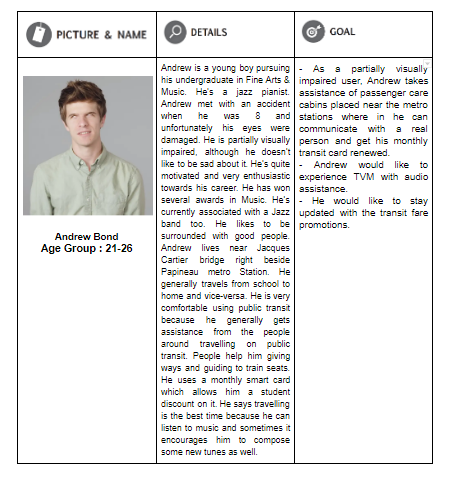
\includegraphics[width=12cm, height=13cm]{Images/Persona_Jatan.png}
  \end{center}
\end{figure}

\begin{figure}[h!]
\begin{center}
  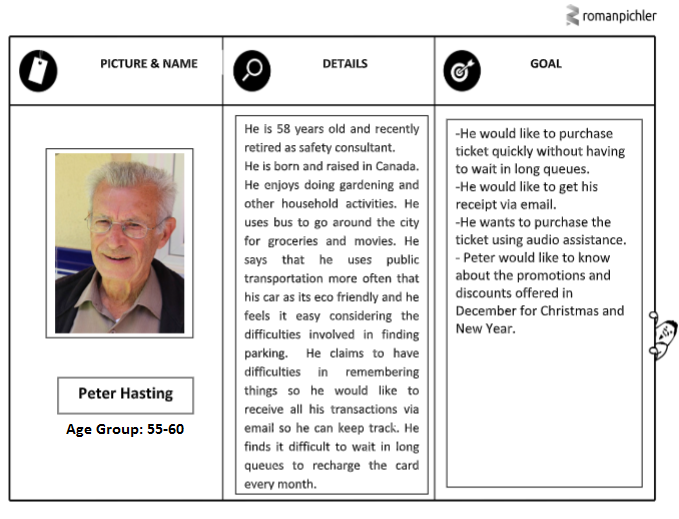
\includegraphics[width=12cm, height=8.8cm]{Images/Persona_Kundana.png}
  \end{center}
\end{figure}

\begin{figure}[h!]
\begin{center}
  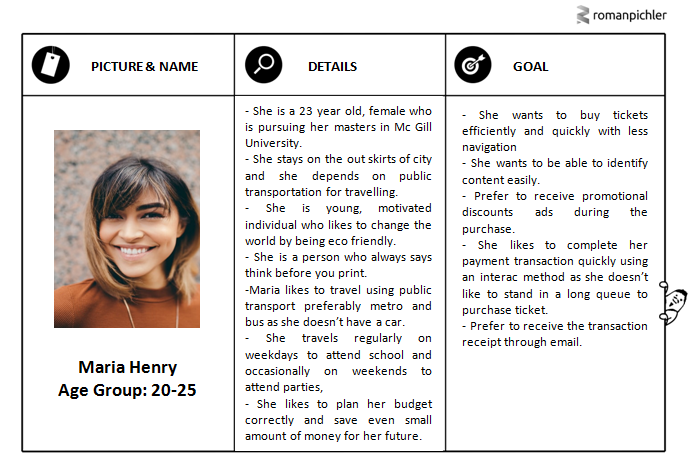
\includegraphics[width=12.5cm, height=8.8cm]{Images/Persona_Surya.png}
  \end{center}
\end{figure}

\begin{figure}[h!]
\begin{center}
  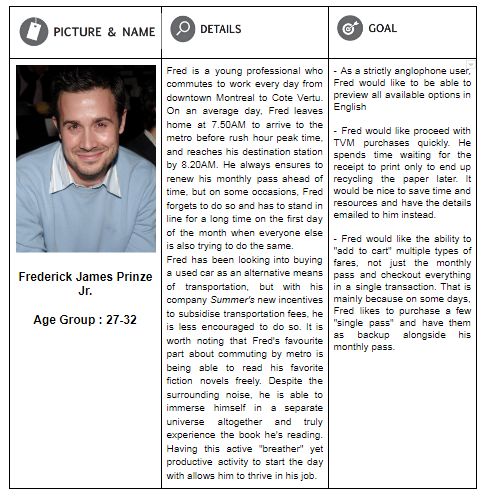
\includegraphics[width=11.5cm, height=13cm]{Images/Persona_Ghalia.png}
  \end{center}
\end{figure}

\begin{figure}[h!]
\begin{center}
  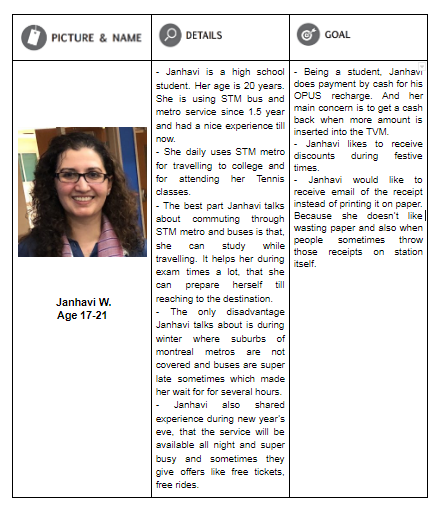
\includegraphics[width=11.5cm, height=13cm]{Images/Persona_Ashutosh.png}
  \end{center}
\end{figure}

\newpage
\subsection{List of User Stories}

\begin{table}[h!]
\centering
\begin{tabular}{|c|l|}
\hline
\textbf{ID}                                                        & TVM\_TC\_001                                                                                                                                                                                                                                                                                                                                              \\ \hline
\textbf{Name}                                                      & Select Available Fares                                                                                                                                                                                                                                                                                                                                    \\ \hline
\textbf{Statement}                                                 & \begin{tabular}[c]{@{}l@{}}\textbf{As :} A user(Maria) \\\textbf{I want :} be able to list all options in terms of available fares\\ \textbf{So that:} I can select the pertinent option.\end{tabular}                                                                                                                                                                                     \\ \hline
\textbf{Constraints}                                               & 1. User can select only one option in the available fare types                                                                                                                                                                                                                                                                                            \\ \hline
\textbf{Priority}                                                  & Medium                                                                                                                                                                                                                                                                                                                                                    \\ \hline
\textbf{Estimation}                                                & 2 Story Points                                                                                                                                                                                                                                                                                                                                            \\ \hline
\textbf{\begin{tabular}[c]{@{}c@{}}Acceptance\\ Test\end{tabular}} & \begin{tabular}[c]{@{}l@{}}1. The User inserts the iGo card in the TVM.\\ 2. Once, the card is authenticated and validated, the system\\ should display a button to redirect to all the fare options.\\ 3. On selection of the button, the available fare options should\\ be displayed with respect to the iGo card inserted by the\\ User.\end{tabular} \\ \hline
\end{tabular}
\end{table}

\begin{table}[h!]
\centering
\begin{tabular}{|c|l|}
\hline
\textbf{ID}                                                        & TVM\_TC\_002                                                                                                                                                                                            \\ \hline
\textbf{Name}                                                      & Select Preferred Language                                                                                                                                                                               \\ \hline
\textbf{Statement}                                                 & \begin{tabular}[c]{@{}l@{}}\textbf{As:} A user(Frederick)\\\textbf{I want:} to change system language \\ \textbf{So that:} I can understand my options.\end{tabular}                                                                         \\ \hline
\textbf{Constraints}                                               & \begin{tabular}[c]{@{}l@{}}The User does not have an option to select a\\ language other than English/French.\end{tabular}                                                                              \\ \hline
\textbf{Priority}                                                  & Medium                                                                                                                                                                                                  \\ \hline
\textbf{Estimation}                                                &  1 Story Points                                                                                                                                                                                                       \\ \hline
\textbf{\begin{tabular}[c]{@{}l@{}}Acceptance\\ Test\end{tabular}} & \begin{tabular}[c]{@{}l@{}}1. The system should display options in English\\  by default.\\ 2. On selection of a preferred language, the options\\  should be displayed in English/French.\end{tabular} \\ \hline
\end{tabular}
\end{table}

\begin{table}[h!]
\centering
\begin{tabular}{|c|l|}
\hline
\textbf{ID}                                                        & TVM\_TC\_003                                                                                                                                                                                             \\ \hline
\textbf{Name}                                                      & Summary of Ticket Purchase                                                                                                                                                                               \\ \hline
\textbf{Statement}                                                 & \begin{tabular}[c]{@{}l@{}}\textbf{As :} A user(Maria)\\ \textbf{I want :} to see the summary of my purchase before finalizing\\ \textbf{So that:} I can confirm correctness.\end{tabular}                                                 \\ \hline
\textbf{Constraints}                                               & \begin{tabular}[c]{@{}l@{}}1.The user should select atleast one fare to display the\\ summary.\end{tabular}                                                                                              \\ \hline
\textbf{Priority}                                                  & Medium                                                                                                                                                                                                   \\ \hline
\textbf{Estimation}                                                & 1 Story Points                                                                                                                                                                                           \\ \hline
\textbf{\begin{tabular}[c]{@{}c@{}}Acceptance\\ Test\end{tabular}} & \begin{tabular}[c]{@{}l@{}}1. The system should display the summary before directing to\\ payment.\\ 2. The TVM should display the fare according to the quantity\\ of fares user selected.\end{tabular} \\ \hline
\end{tabular}
\end{table}

\begin{table}[h!]
\centering
\begin{tabular}{|c|l|}
\hline
\textbf{ID}                                                        & TVM\_TC\_004                                                                                                                                                                                                                                                                                                                                                                                                                                                                            \\ \hline
\textbf{Name}                                                      & Choose Payment using card (Debit/Credit/Interac)                                                                                                                                                                                                                                                                                                                                                                                                                                        \\ \hline
\textbf{Statement}                                                 & \begin{tabular}[c]{@{}l@{}}\textbf{As:} A user(Frederick)\\ \textbf{I want:} choose to make a payment by card (Interac \\ /credit / debit)\\ \textbf{So that:} I can conveniently pay and complete transaction\end{tabular}                                                                                                                                                                                                                                                                                                   \\ \hline
\textbf{Constraints}                                               & \begin{tabular}[c]{@{}l@{}}1. Credit Cards accepted are only Master credit card and \\ Visa credit card.\\ 2. Debit Cards accepted are only those issued by\\ Canadian Banks.\\ 3. Cards should have an Interac functionality enabled.\\ 4. The currency accepted is CAD only.\end{tabular}                                                                                                                                                                                             \\ \hline
\textbf{Priority}                                                  & High                                                                                                                                                                                                                                                                                                                                                                                                                                                                                    \\ \hline
\textbf{Estimation}                                                & 8 Story Points                                                                                                                                                                                                                                                                                                                                                                                                                                                                                        \\ \hline
\textbf{\begin{tabular}[c]{@{}c@{}}Acceptance\\ Test\end{tabular}} & \begin{tabular}[c]{@{}l@{}}1. The User has selected either the tickets or the Smart \\ card recharge option and is required to pay the \\ corresponding fee.\\ 2. The User selects card (credit/debit/Interac) as\\ method of payment when prompted by TVM.\\ 3. The card (credit/debit/Interac) inserted is valid.\\ 4. The card (credit/debit) PIN entered is valid. \\ 5. The payment transaction is validated, approved by\\  the Bank gateway and received by the TVM\end{tabular} \\ \hline
\end{tabular}
\end{table}

\begin{table}[h!]
\centering
\begin{tabular}{|c|l|}
\hline
\textbf{ID}                                                        & TVM\_TC\_005                                                                                                                                                                                                                                                                                        \\ \hline
\textbf{Name}                                                      & Select Payment by Cash                                                                                                                                                                                                                                                                              \\ \hline
\textbf{Statement}                                                 & \begin{tabular}[c]{@{}l@{}}\textbf{As :} A user(Janhavi)\\ \textbf{I want :} to make a payment by cash\\ \textbf{So that:} I can conveniently purchase the ticket.\end{tabular}                                                                                                                                                         \\ \hline
\textbf{Constraints}                                               & \begin{tabular}[c]{@{}l@{}}1. The User cannot insert other currencies apart from\\ Canadian dollars.\\ 2. The User cannot insert fake currency.\\ 3. The User Should have enough money to complete the\\ transaction\end{tabular}                                                                   \\ \hline
\textbf{Priority}                                                  & High                                                                                                                                                                                                                                                                                                \\ \hline
\textbf{Estimation}                                                & 5 Story Points                                                                                                                                                                                                                                                                                      \\ \hline
\textbf{\begin{tabular}[c]{@{}c@{}}Acceptance\\ Test\end{tabular}} & \begin{tabular}[c]{@{}l@{}}1. After the User has selected “Pay by Cash”, the system\\ should show the amount due and accept Canadian currency\\ only.\\ 2. The User inserts the cash and TVM accepts the same.\\ 3. After all the validations, TVM returns if there’s any cash\\ back.\end{tabular} \\ \hline
\end{tabular}
\end{table}


\begin{table}[h!]
\centering
\begin{tabular}{|c|l|}
\hline
\textbf{ID}                                                        & TVM\_TC\_006                                                                                                                                                                                                                                                                                                                                                                 \\ \hline
\textbf{Name}                                                      & Print Receipt of Ticket Purchase                                                                                                                                                                                                                                                                                                                                             \\ \hline
\textbf{Statement}                                                 & \begin{tabular}[c]{@{}l@{}}\textbf{As :} A user(Peter)\\ \textbf{I want :} to print receipt of my purchase \\ \textbf{So that:} I can track my records.\end{tabular}                                                                                                                                                                                                                                           \\ \hline
\textbf{Constraints}                                               & \begin{tabular}[c]{@{}l@{}}1.The user must complete ongoing transaction before \\ requesting to print receipt.\\ 2. TVM contains blank cards/papers to print the receipt\end{tabular}                                                                                                                                                                                        \\ \hline
\textbf{Priority}                                                  & Medium                                                                                                                                                                                                                                                                                                                                                                         \\ \hline
\textbf{Estimation}                                                & 2 Story Points                                                                                                                                                                                                                                                                                                                                                               \\ \hline
\textbf{\begin{tabular}[c]{@{}c@{}}Acceptance\\ Test\end{tabular}} & \begin{tabular}[c]{@{}l@{}}1. Once transaction completes,  TVM will prompt option \\ to user whether to print receipt or not.\\ 2. If user selects to print the receipt detailing the transaction\\ parameters as Data \& Time, Ticket Type, Amount, \\ Payment Mode\\ 3. TVM must not print the receipt, if user select option\\  as not to print the receipt.\end{tabular} \\ \hline
\end{tabular}
\end{table}

\begin{table}[h!]
\centering
\begin{tabular}{|c|l|}
\hline
\textbf{ID}                                                        & TVM\_TC\_007                                                                                                                                                                                                                                                                                                     \\ \hline
\textbf{Name}                                                      & Enable audio assistance                                                                                                                                                                                                                                                                                          \\ \hline
\textbf{Statement}                                                 & \begin{tabular}[c]{@{}l@{}}\textbf{As :} A visually-impaired user(Andrew)\\ \textbf{I want :} enable audio assistance\\ \textbf{So that:} I can conveniently listen to and understand all my\\ options\end{tabular}                                                                                                                                 \\ \hline
\textbf{Constraints}                                               & \begin{tabular}[c]{@{}l@{}}1. Output audio from the physical TVM is tuned to an \\ optimal volume which may be deemed low in a \\ crowded public setting.\\ 2. Audio sentences may not be rewound once they are said.\\ 3. The voice assistant may not be able to adequately process\\ voice input.\end{tabular} \\ \hline
\textbf{Priority}                                                  & Medium                                                                                                                                                                                                                                                                                                           \\ \hline
\textbf{Estimation}                                                & 5 Story Points                                                                                                                                                                                                                                                                                                   \\ \hline
\textbf{\begin{tabular}[c]{@{}c@{}}Acceptance\\ Test\end{tabular}} & \begin{tabular}[c]{@{}l@{}}1. The User is able to request voice assistant and receive initial\\ guidance.\\ 2. The User hears and understands the response from the\\ TVM.\\ 3. The TVM hears and understands the requests from the user.\end{tabular}                                                           \\ \hline
\end{tabular}
\end{table}

\begin{table}[h!]
\centering
\begin{tabular}{|c|l|}
\hline
\textbf{ID}                                                        & TVM\_TC\_008                                                                                                                                                                                                                                                                                                            \\ \hline
\textbf{Name}                                                      & System Maintenance                                                                                                                                                                                                                                                                                                      \\ \hline
\textbf{Statement}                                                 & \begin{tabular}[c]{@{}l@{}}\textbf{As :} A System(TVM) Maintainer (Operator) \\ \textbf{I want :}I want to be able to configure the system \\ \textbf{So that :} TVM captures the latest fares and offered trips\end{tabular}                                                                                                                                 \\ \hline
\textbf{Constraints}                                               & \begin{tabular}[c]{@{}l@{}}1. Maintainer must have access to secured storage areas of \\ TVM wherein money, tickets and blank cards for printing\\  receipts are stored.\\ 2. Maintainer must have authority to power off the TVM\end{tabular}                                                                          \\ \hline
\textbf{Priority}                                                  & High                                                                                                                                                                                                                                                                                                                    \\ \hline
\textbf{Estimation}                                                & 5 Story Points                                                                                                                                                                                                                                                                                                          \\ \hline
\textbf{\begin{tabular}[c]{@{}c@{}}Acceptance\\ Test\end{tabular}} & \begin{tabular}[c]{@{}l@{}}1. TVM must verify maintainers credentials/details before\\ allowing access to secure storage area. \\ 2. TVM must display the status, when maintainers completes\\  loading of tickets, inserting blank cards for printing receipts,\\  collecting money and configure changes\end{tabular} \\ \hline
\end{tabular}
\end{table}

\begin{table}[h!]
\centering
\begin{tabular}{|c|l|}
\hline
\textbf{ID}                                                        & TVM\_TC\_009                                                                                                                                                                         \\ \hline
\textbf{Name}                                                      & Use invalid credit card                                                                                                                                                              \\ \hline
\textbf{Statement}                                                 & \begin{tabular}[c]{@{}l@{}}\textbf{As:} A bad user (Crook) \\ \textbf{I should not:} use an invalid credit card to make a payment\\ \textbf{So that:} I do not circumvent the security of the TVM.\end{tabular}         \\ \hline
\textbf{Constraints}                                               & \begin{tabular}[c]{@{}l@{}}The User can use any credit card (stolen or not) so long as it is\\ valid in terms of information and expiration date.\end{tabular}                       \\ \hline
\textbf{Priority}                                                  & High                                                                                                                                                                                 \\ \hline
\textbf{Estimation}                                                & 8 Story Points                                                                                                                                                                       \\ \hline
\textbf{\begin{tabular}[c]{@{}c@{}}Acceptance\\ Test\end{tabular}} & \begin{tabular}[c]{@{}l@{}}1. The system should validate payment method.\\ 2. On insertion of an invalid credit card, the transaction should\\ immediately be rejected.\end{tabular} \\ \hline
\end{tabular}
\end{table}

\begin{table}[h]
\centering
\begin{tabular}{|c|l|}
\hline
\textbf{ID}                                                        & TVM\_TC\_010                                                                                                                                                                               \\ \hline
\textbf{Name}                                                      & Manipulate the fares                                                                                                                                                                       \\ \hline
\textbf{Statement}                                                 & \begin{tabular}[c]{@{}l@{}}\textbf{As :} A bad user (Crook)\\ \textbf{I want :} should not be able to make config changes\\ \textbf{So that:} it would impact the users and owners of the system.\end{tabular}                \\ \hline
\textbf{Constraints}                                               & \begin{tabular}[c]{@{}l@{}}The user(bad) tries to use any credentials to login to the\\ server without undergoing authentication.\end{tabular}                                             \\ \hline
\textbf{Priority}                                                  & High                                                                                                                                                                                       \\ \hline
\textbf{Estimation}                                                & 3 Story Points                                                                                                                                                                             \\ \hline
\textbf{\begin{tabular}[c]{@{}c@{}}Acceptance\\ Test\end{tabular}} & \begin{tabular}[c]{@{}l@{}}1. TVM should not allow the hacker to change the fare details.\\ 2.TVM should show error message when a hacker is trying to\\ login to the server.\end{tabular} \\ \hline
\end{tabular}
\end{table}

\newpage
\section{Traceability Matrix}
\paragraph{} The traceability matrix for user stories describes the tracing of every feature back to its associated requirement. It represents tracing each requirement back to its sources. Backward traceability also helps in verifying that the user stories are in scope with other requirement artifacts.
\paragraph{} The Traceability Matrix for all user stories is presented in the table below. 

\begin{table}[h]
\centering
\begin{tabular}{|l|c|c|c|c|c|}
\hline
\multicolumn{1}{|c|}{\textbf{\begin{tabular}[c]{@{}c@{}}User story\\  ID\end{tabular}}} & \textbf{\begin{tabular}[c]{@{}c@{}}UseCase \\ Model\end{tabular}} & \textbf{\begin{tabular}[c]{@{}c@{}}Domain \\ Model\end{tabular}} & \textbf{\begin{tabular}[c]{@{}c@{}}User \\ Story\end{tabular}} & \textbf{Interview} & \textbf{Constraints} \\ \hline
TVM\_TC\_001                                                                            & \checkmark                                                                 &                                                                 &                                                               &\checkmark                  &                     \\ \hline
TVM\_TC\_002                                                                            & \checkmark                                                                 & \checkmark                                                                &                                                               &                   &                     \\ \hline
TVM\_TC\_003                                                                            &                                                                 &                                                                 &                                                             & \checkmark                  &                     \\ \hline
TVM\_TC\_004                                                                            & \checkmark                                                                 & \checkmark                                                                &                                                               & \checkmark                  &                     \\ \hline
TVM\_TC\_005                                                                            & \checkmark                                                                 & \checkmark                                                                &                                                               &                   &                     \\ \hline
TVM\_TC\_006                                                                            & \checkmark                                                                 & \checkmark                                                                &                                                               & \checkmark                  &                     \\ \hline
TVM\_TC\_007                                                                            & \checkmark                                                                 & \checkmark                                                                &                                                               & \checkmark                  &                     \\ \hline
TVM\_TC\_008                                                                            & \checkmark                                                                &                                                                 &                                                               &                   & \checkmark                    \\ \hline
TVM\_TC\_009                                                                            & \checkmark                                                                &                                                                 & \checkmark                                                              &                   & \checkmark                    \\ \hline
TVM\_TC\_010                                                                            &\checkmark                                                                 &                                                                 & \checkmark                                                              &                   & \checkmark                    \\ \hline
\end{tabular}
\end{table}


\section{Implementation of User Stories}
\paragraph{} As part of implementation to ensure the realizable of each user stories, each member implemented below user stories and tested for the acceptance criteria.

Source Code are available in the below path:
\url{https://drive.google.com/drive/folders/1E3WD97q2F1XtsizKSM72uXV-VEQ8B_Hn?usp=sharing}

\begin{table}[h]
\centering
\begin{tabular}{|c|c|}
\hline
\textbf{User Story ID} & \textbf{Implemented By} \\ \hline
TVM\_TC\_009           & Jatan Gohel             \\ \hline
TVM\_TC\_002           & Ghalia ElKerdi          \\ \hline
TVM\_TC\_003           & Surya Prakash           \\ \hline
TVM\_TC\_004           & Kundana Gangam          \\ \hline
TVM\_TC\_005           & Ashutosh Ramesh         \\ \hline
\end{tabular}
\end{table}

\begin{thebibliography}{9}


\bibitem{wiki} 
Persona Template
\\\texttt{https://www.romanpichler.com/tools/the-persona-template/}

\bibitem{Ticket Vending Machine} 
Wikipedia,
\\\texttt{https://en.wikipedia.org/wiki/Ticket\_machine}

\bibitem{} 
T-12 -Transport Act - Government of Quebec,
\\\texttt{http://legisquebec.gouv.qc.ca/en/ShowDoc/cs/T\-12}

\bibitem{} 
Quebec Public Transport Policy - Government of quebec.
\\\texttt{http://www.bv.transports.gouv.qc.ca/mono/0926032.pdf}


\bibitem{ATM} 
ATM Stimulation by R. C. Bjork,
\\\texttt{http://www.cs.gordon.edu/courses/cs211/ATMExample/index.html}

\bibitem{ATM} 
The Art of Asking: Ask Better Questions, 
Get Better Answers. By T. J. Fadem. FT Press. 2009
\\\texttt{}

\bibitem{ATM} 
Object-Oriented Software Engineering: Practical Software Development using UML and Java. By T. C. Lethbridge, R. Laganière. McGraw-Hill. 2005.
\\\texttt{}

\bibitem{ATM} 
Estimation using Planning Poker Technique.
\\\texttt{https://www.mountaingoatsoftware.com/agile/planning-poker}



\end{thebibliography}
\addcontentsline{toc}{section}{References}

\end{document}
